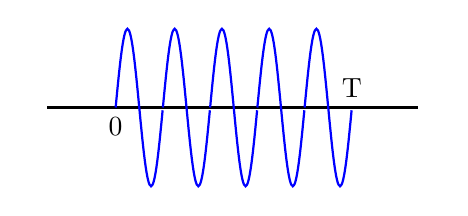
\begin{tikzpicture}[-,shorten >=1pt,auto,node distance=2cm,
  thick,main node/.style={circle,fill=black,draw,font=\sffamily\Large\bfseries}]

\usetikzlibrary{calc}
  
  \node[] (-1) {};
  \node[] (0) [right of=-1, node distance=1cm] {};
  \node[] (T) [right of=0, node distance=3cm] {};
  \node[] (2) [right of=T, node distance=1cm] {};
  
  \node[] at (0) [below] {0};
  \node[] at (T) [above] {T};

  \path[every node/.style={font=\sffamily\small}]
    (-1) edge node {} (2);
  
  \pgfmathsetmacro\K{5}
  \pgfmathsetmacro\k{(\K -1)}
  \pgfmathsetmacro\T{(3 / \K)}
  \pgfmathsetmacro\t{(1 / 4)}
  
  
  \foreach \x in {0,...,\k}
  {\draw[thick, blue]
    ($(0)+(\T*\x,0)$) sin ($(0)+(\T*\x+\t*\T,1)$) cos ($(0)+(\T*\x+2*\t*\T,0)$) sin ($(0)+(\T*\x+3*\t*\T,-1)$) cos ($(0)+(\T*\x+4*\t*\T,0)$);}

\end{tikzpicture}